\documentclass[11pt]{article}
\usepackage{amsmath, amsfonts, amssymb,amsthm}
\usepackage[includeheadfoot]{geometry} % For page dimensions
\usepackage{fancyhdr}
\usepackage{enumerate} % For custom lists
\usepackage{tikz-cd}
\usepackage{xr}
\externaldocument{427Notes}

\fancyhf{}
\lhead{427 Exercises}
\rhead{Tighe McAsey}
\pagestyle{fancy}

% Page dimensions
\geometry{a4paper, margin=1in}

\theoremstyle{definition}
\newtheorem{pb}{}

% Commands:

\newcommand{\set}[1]{\{#1\}}
\newcommand{\abs}[1]{\lvert#1\rvert}
\newcommand{\norm}[1]{\lvert\lvert#1\rvert\rvert}
\newcommand{\gen}[1]{\left\langle #1 \right\rangle}
\newcommand{\tand}{\text{ and }}
\newcommand{\tor}{\text{ or }}
\newcommand{\falg}{F^{\text{alg}}}
\newcommand{\gal}{\text{Gal}}
\newcommand{\mor}{\text{Mor}}
\newcommand{\floor}[1]{\left\lfloor #1 \right\rfloor}
\newcommand{\im}{\text{Im}}
\title{Exercises}

\begin{document}
\maketitle

\section{Categories and Pre-reqs}

\emph{exercise - }\label{PreEx1} Show the forgetful functor \(F: \text{Vect}_k \to \text{Set}\) is a functor.

\emph{proof - } The identity linear transformation is the identity when regarded as a set mapping, if \(T: U \to V, \varphi: V \to S\) as vector spaces, then \(F(\varphi)\circ F(T)\) is a well defined set mapping, which maps \(U \to S\) as sets.

%%%%%%%%%%%%%%%%%%%%%%%%%%%%%%%%%%%%%%%%%%%%%%%%%%%%%%%%%%%%%%%%%%%%%%%%%%%%%%%%%%%%%%%%%%%%%%%%%%%%%%%%%%%%%%%%%%%%%%%%%%%%%%%%%%%%%%%
%%%%%%%%%%%%%%%%%%%%%%%%%%%%%%%%%%%%%%%%%%%%%%%%%%%%%%%%%%%%%%%%%%%%%%%%%%%%%%%%%%%%%%%%%%%%%%%%%%%%%%%%%%%%%%%%%%%%%%%%%%%%%%%%%%%%%%%

\section{Chain Complexes}\label{CCEx} \ref{CCNotes}

\emph{exercise - }\label{CCEx1} Show that \(\mathbf{h} = (h_i)\), \(h_i: C_i \to C_{i+1}'\), then \(h_{i-1}\circ d_i + d_{i+1}' \circ h_i\) is a chain map.

\emph{proof - } We need to check that \(d_i' \circ f_i = f_{i-1} \circ d_i\), in other words we need to show
\begin{align*}
    d_i' \circ (h_{i-1}\circ d_i + d_{i+1}' \circ h_i) = (h_{i-2}\circ d_{i-1} + d_{i}' \circ h_{i-1})\circ d_i
\end{align*}
Since we are in a module, we can distribute \(d_i'\) on the left hand side, rewriting the condition as
\begin{align*}
    d_i' \circ h_{i-1}\circ d_i + d_i' \circ d_{i+1}' \circ h_i = h_{i-2}\circ d_{i-1}\circ d_i + d_{i}' \circ h_{i-1}\circ d_i
\end{align*}
So it will suffice to show that
\begin{align*}
    d_i' \circ d_{i+1}' \circ h_i = h_{i-2}\circ d_{i-1}\circ d_i
\end{align*}
But this is trivial since "\(d^2 = 0\)"


%%%%%%%%%%%%%%%%%%%%%%%%%%%%%%%%%%%%%%%%%%%%%%%%%%%%%%%%%%%%%%%%%%%%%%%%%%%%%%%%%%%%%%%%%%%%%%%%%%%%%%%%%%%%%%%%%%%%%%%%%%%%%%%%%%%%%%%


\emph{exercise - }\label{CCEx2} A homotopy of chains is an equivalence relation

\emph{proof - } We will prove the following items: reflexivity, symmetry, transitivity
\begin{itemize}
    \item To see that \(f \sim f\), take each to be the zero map, \(h_i = 0, \forall i\). In this case the diagram with maps given by \(\mathbf{h}\) is immediate.
    \item Suppose that \(f \sim g\), then we have some \(\mathbf{h}\), such that \(g_i -f_i = h_{i-1}\circ d_i + d_{i+1}' \circ h_i\) for each \(i\). Since \(h_i\) are morphisms of modules, so are \(-h_i\), so in particular we have \(\mathbf{-h} := (-h_i)_i\), so that 
    \begin{align*}
        f_i - g_i &= -(g_i - f_i) = -(h_{i-1}\circ d_i + d_{i+1}' \circ h_i) = -h_{i-1}\circ d_i + -d_{i+1}' \circ h_i \\
        &= -h_{i-1}\circ d_i + d_{i+1}' \circ -h_i
    \end{align*}
    The last line follows since \(d_{i+1}'\) is linear.
    \item Suppose that \(f \sim g \sim r\), and let \(\mathbf{h, k}\) be respective witnesses of these homotopies. Then we have
    \begin{align*}
            &r_i - g_i = k_{i-1}\circ d_i + d_{i+1}'\circ k_i \\
            &g_i - f_i = h_{i-1}\circ d_i + d_{i+1}'\circ h_i
    \end{align*}
    This furnishes
    \begin{align*}
        &r_i - f_i = k_{i-1}\circ d_i + d_{i+1}'\circ k_i + h_{i-1}\circ d_i + d_{i+1}'\circ h_i
                   = (k_{i-1} + h_{i-1})\circ d_i + d_{i+1}'\circ(h_i + k_i)
    \end{align*}
    So we have the homotopy \(r \sim f\) via \(\mathbf{h} + \mathbf{k}\), we are done since we already proved symmetry.
\end{itemize}


%%%%%%%%%%%%%%%%%%%%%%%%%%%%%%%%%%%%%%%%%%%%%%%%%%%%%%%%%%%%%%%%%%%%%%%%%%%%%%%%%%%%%%%%%%%%%%%%%%%%%%%%%%%%%%%%%%%%%%%%%%%%%%%%%%%%%%%


\emph{exercise - }\label{CCEx3} Show that the following two chain complexes are homotopic:
\begin{equation*}
    \begin{tikzcd}
        0 \arrow[r] & \mathbf{Z} \oplus \mathbf{Z} \arrow[r,"{(\cdot , 2\cdot)}"] & \mathbf{Z} \oplus \mathbf{Z} \arrow[r] & 0 \oplus \mathbf{Z}/(2) \arrow[r] & 0 \\
        0 \arrow[r] & \mathbf{Z} \arrow[r,"2\cdot"] & \mathbf{Z} \arrow[r] & \mathbf{Z}/(2) \arrow[r] & 0
    \end{tikzcd}
\end{equation*}

\emph{proof - } Let each \(f_i\) be the projection of the second coordinate, and each \(g_i\) the inclusion into the second coordinate. In thise case we have
\begin{align*}
    \mathbf{1}_{C'} - \mathbf{fg} = \mathbf{0}
\end{align*}
and hence \(\mathbf{h} = (0)_i\) witnesses the homotopy. The slightly harder case is the other direction. Define \(h_2 = h_0 = h_{-1} = 0\), and \(h_1: (m,n) \mapsto m\). By definition of \(\mathbf{f}, \mathbf{g}\), we have \(1_{C,i} - g_if_i: (m,n) \mapsto (m,0)\), so we just need to check that our given \(\mathbf{h}\) satisfies this.
\begin{align*}
    &(d_3h_2 + h_1d_2)(m,n) = 0 + h_1(m,2n) = (m,0) \\
    &(d_2h_1 + h_0d_1)(m,n) = d_2(m,0) + 0 = (m,0) \\
    &(d_1h_0 + h_{-1}d_0)(0,n) = 0 + 0 = (0,0)
\end{align*}
This verifies the homotopy.


%%%%%%%%%%%%%%%%%%%%%%%%%%%%%%%%%%%%%%%%%%%%%%%%%%%%%%%%%%%%%%%%%%%%%%%%%%%%%%%%%%%%%%%%%%%%%%%%%%%%%%%%%%%%%%%%%%%%%%%%%%%%%%%%%%%%%%%


\textbf{Theorem - }\label{CCEx4} ("\emph{The Fundamental Theorem of Homology For Chain Complexes}") If chain complexes \(C,C'\) are homotopic, then they have the same Homology Modules.

\emph{proof - } Recall that
\begin{align*}
    H^i := \frac{\ker(d_i)}{\im(d_{i+1})}
\end{align*}
Now let the homotopy be given by \(\mathbf{f}:C \to C', \mathbf{g}:C' \to C\), there is a natural induced map of \(f_i\) on \(H^i\), given by restricting \(f_i\) to \(\im(d_{i+1})\), then taking the unique map from the quotient by the kernel of \(d_i\), which exists and is unique by the first isomorphism theorem. Calling this induced map \(f_{i,*}\), we need to check that
\(f_{i,*}\) maps into \(H_i'\). First it is immediate that \(f_i\vert_{\ker{d_i}}: \ker d_i \to \ker d_i'\), since \(d_i'f_i = f_{i-1}d_i\), where the right hand side is zero when restricted to \(\ker(d_i)\).

\textcolor{red}{TODO -- Finish proof}


%%%%%%%%%%%%%%%%%%%%%%%%%%%%%%%%%%%%%%%%%%%%%%%%%%%%%%%%%%%%%%%%%%%%%%%%%%%%%%%%%%%%%%%%%%%%%%%%%%%%%%%%%%%%%%%%%%%%%%%%%%%%%%%%%%%%%%%
%%%%%%%%%%%%%%%%%%%%%%%%%%%%%%%%%%%%%%%%%%%%%%%%%%%%%%%%%%%%%%%%%%%%%%%%%%%%%%%%%%%%%%%%%%%%%%%%%%%%%%%%%%%%%%%%%%%%%%%%%%%%%%%%%%%%%%%


\section{Homology and Cell Complexes}

\emph{exercise - }\label{HEx1} Let \(G\) be a graph, then \(\ker d_1 = \set{\text{Cycles in }G}\)

\emph{proof - } We have the map \(d_1: \oplus_i \mathbf{Z}e_i \to \oplus_i \mathbf{Zv_i}\), then \(\sum_i k_i e_i \in \ker d_1 \iff \sum_i k_i (H(e_i) - T(e_i)) = 0\), where \(H(e)\) denotes the target of an edge, and \(T(e)\) denotes the source of an edge. Then \(\sum_i k_i (H(e_i) - T(e_i)) = \sum_j\ell_j v_j = 0 \iff \ell_j = 0,\; \forall j\). Where \(\ell_j = \sum_{\set{e_i \mid v_j = H(e_i)}} k_i - \sum_{\set{e_i \mid v_j = T(e_i)}} k_i\) so that \(\ell_j = 0\) for all \(j\) exactly when every vertex has an equal number of in and out edges.

%%%%%%%%%%%%%%%%%%%%%%%%%%%%%%%%%%%%%%%%%%%%%%%%%%%%%%%%%%%%%%%%%%%%%%%%%%%%%%%%%%%%%%%%%%%%%%%%%%%%%%%%%%%%%%%%%%%%%%%%%%%%%%%%%%%%%%%

\emph{exercise - }\label{HEx2} Show that for the graph \(G\), with \(V(G) = \set{x,y}, E(G) = \set{a = (x,y),b = (x,y), c = (x,y)}\) we have \(\ker d_1 = \gen{a-b, b-c}\)

\emph{proof - } Here we have \(d_1: a,b,c \mapsto y-x\), then \(a-b, b-c \in \ker d_1\). We have \(d_1: n_1a + n_2b + n_3c \mapsto (n_1 + n_2 + n_3)(x-y)\), so that \(\ker d_1 = \set{na + mb + k\ell \mid n + m + \ell = 0}\), so fixing \(na + mb + k\ell = na + mb + -(n+m)c \in \ker d_1\), we have \(na + mb + k\ell = n(a-b) + (m+n)(b-c) \in (a-b,b-c)\)

%%%%%%%%%%%%%%%%%%%%%%%%%%%%%%%%%%%%%%%%%%%%%%%%%%%%%%%%%%%%%%%%%%%%%%%%%%%%%%%%%%%%%%%%%%%%%%%%%%%%%%%%%%%%%%%%%%%%%%%%%%%%%%%%%%%%%%%

\emph{exercise - }\label{HEx3} Consider the following Graph:

\begin{equation}
        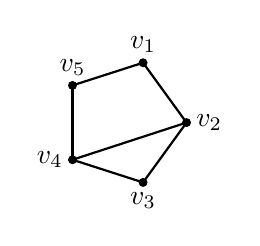
\begin{tikzpicture}[scale=0.8]
                \coordinate (b) at (0.31,0.95);
                \coordinate (c) at (1,0);
                \coordinate (d) at (0.31,-0.95);
                \coordinate (e) at (-0.81,-0.59);
                \coordinate (f) at (-0.81,0.59);
    
                \draw[fill] (b) circle (1.75pt);
                \draw[fill] (c) circle (1.75pt);
                \draw[fill] (d) circle (1.75pt);
                \draw[fill] (e) circle (1.75pt);
                \draw[fill] (f) circle (1.75pt);
    
                \draw[thick] (b)--(c);
                \draw[thick] (c)--(d);
                \draw[thick] (d)--(e);
                \draw[thick] (e)--(f);
                \draw[thick] (b)--(f);
                \draw[thick] (c)--(e);
                
                \node[above] at (0.31,0.95) {\(v_1\)};
                \node[right] at (1,0) {\(v_2\)};
                \node[below] at (0.31,-0.95) {\(v_3\)};
                \node[left] at (-0.81,-0.59) {\(v_4\)};
                \node[above] at (-0.81,0.59) {\(v_5\)};
    \end{tikzpicture}
    \end{equation}

    Where the edges are oriented with the larger vertex index at the head and smaller at the tail. Compute generators for the cycles, and show that \(C_*(G) \simeq C_*(G')\) as chain complexes, where \(G'\) is \(G\) with \((v_1,v_5)\) replaced with \((v_5,v_1)\). Finally, show that \(H_1(G) \cong H_1(G')\)
    
    \emph{proof - }
    We can write \(d_1\) as a matrix,
    \begin{align*}
        \begin{bmatrix} -1 & 0 &0 &0 &0 &-1 \\ 1 &-1 &-1 &0 &0 &0  \\ 0 & 1& 0&-1&0 &0  \\ 0 &0 &1 &1 &-1 &0 \\ 0 & 0&0 &0 & 1& 1 \end{bmatrix} \overset{\text{Row Reduction}}{\rightsquigarrow} \begin{bmatrix} -1&0&0&0&0&-1\\0&-1&-1&0&0&-1\\0&0&-1&-1&0&-1\\0&0&0&0&-1&-1\\0&0&0&0&0&0\end{bmatrix}
    \end{align*}
    So the kernel has rank 2.
    From this matrix we can compute generators for the kernel, (and thus the cycles)
    \[\ker d_1 = (e_2-e_4,e_1+e_5-e_6)\]

    To show that \(C_*(G)\), and \(C_*(G')\) are chain homotopic, define \[f:v_i \mapsto v_i', e_i \mapsto e_i', \quad g: v_i' \mapsto v_i, e_i' \mapsto e_i\].
    By construction these are chain maps, since firstly \(d_0 = 0, d_0' = 0\), and \(e_i = e_i'\) for each \(e_i \neq (v_1,v_5)\), and the values of \(d_1\) agree with \(d_1'\) on each of the equal \(e_i = e_i'\). For \(e = (v_1,v_5), e' = (v_5,v_1)\), we have \(f_1(e) = -e',g_1(e')=-e\), for \(e \neq (v_1,v_5), e' \neq (v_5,v_1)\) commutativity is obvious since \(d(e) = d'(e')\) in this case. For \(e = (v_1,v_5)\) we have \(f_0 \circ d(e) = f_0(x-y) = x-y = -(y-x) = -d_1'(e') = d_1'(f_1(e))\), the argument is the exact same for commutativity of the square replacing \(g\) for \(f\) and \(e'\) for \(e\). Then \(f \circ g = 1\), so we can just choose our homotopy to be the zero map.

    To see that the homology is the same, there are 2 possible solutions both are easy. The first is that they are isomorphic as chain complexes, the second is that \(d_1\) is rewritten by multiplying a row by \(-1\), preserving the row reduced form and hence the generators of the kernel.



    %%%%%%%%%%%%%%%%%%%%%%%%%%%%%%%%%%%%%%%%%%%%%%%%%%%%%%%%%%%%%%%%%%%%%%%%%%%%%%%%%%%%%%%%%%%%%%%%%%%%%%%%%%%%%%%%%%%%%%%%%%%%%%%%%%%%%%%

    
    \emph{exercise - }\label{HEx4} Let \(\Gamma, \Gamma'\) be arbitrary graphs such that \(\Gamma \simeq \Gamma'\), then \(C_*(\Gamma) \simeq C_*(\Gamma')\)

    \emph{proof - } In (i) we show that homotopy of graphs is independent of orientation, and in (ii), we show that it is equivalent up to quotienting by an edge between to vertices, this is sufficient since it allows us to show that (since the graphs are homotopic they have the same Euler characteristic)
    \[C_*(\Gamma) \simeq C_*(\bigvee_{1 \leq k \leq \chi(\Gamma)} S^1) \simeq C_*(\Gamma')\]

    (i) Assume that \(\Gamma\setminus e_0 = \Gamma' \setminus e_0'\), such that \(e_0' = -e_0\), we copy the proof in the previous question.
    \begin{align*}
        f: &C_*(\Gamma) \to C_*(\Gamma')
        &\begin{cases}
            e_0 \mapsto -e_0' \\
            e_i \mapsto e_i' & i \geq 1 \\
            v_i \mapsto v_i'
        \end{cases}
        g: &C_*(\Gamma') \to C_*(\Gamma)
        &\begin{cases}
            e_0' \mapsto -e_0 \\
            e_i' \mapsto e_i & i \geq 1 \\
            v_i' \mapsto v_i
        \end{cases}
    \end{align*}
    \(fg = 1_{C_*(\Gamma)}\), \(gf = 1_{C_*(\Gamma')}\), so they are homotopies so long as they are chain maps. This is trivial except for the "square" where edges map to vertices.
    Commutativity on generators is trivial apart from \(e_0\), and \(e_0'\), in this case \(f\circ d_1(e_0) = f(v_1 - v_0) = v_1' - v_0' = -(v_0' - v_1') = d_1'(-e_0') = d_1'\circ f (e_0)\). The proof is the same for \(g\).

    (ii) \textcolor{red}{TODO!!}

    %%%%%%%%%%%%%%%%%%%%%%%%%%%%%%%%%%%%%%%%%%%%%%%%%%%%%%%%%%%%%%%%%%%%%%%%%%%%%%%%%%%%%%%%%%%%%%%%%%%%%%%%%%%%%%%%%%%%%%%%%%%%%%%%%%%%%%%


    \emph{exercise - }\label{HEx5} Using the cell structures for \(S^2\) from \(e^2 \cup e^0\), \(e^2 \cup e^2 \cup e^1 \cup e^0\) Build \(C_*(S^2)\) and compute its Homology.

    \emph{proof - } The first cell structure gives the sequence

    \begin{equation*}
        \begin{tikzcd}
            0 \arrow[r] & \mathbb{Z} \arrow[r] & 0 \arrow[r] & \mathbb{Z} \arrow[r] & 0
        \end{tikzcd}
    \end{equation*}

    In this case the homology modules are trivially \(H_i(C_*(S^2)) = \begin{cases}
        0 & i \neq 0,2 \\
        1 & i = 0,2
    \end{cases}\)

    The second cell structure gives the sequence

    \begin{equation*}
        \begin{tikzcd}
            0 \arrow[r] & \mathbb{Z}e_0^2 \oplus \mathbb{Z}e_1^2 \arrow[r,"{d_2}"] & \mathbb{Z}e_0^1 \arrow[r,"{d_1}"] & \mathbb{Z}e_0^0 \arrow[r] & 0
        \end{tikzcd}
    \end{equation*}

    Where \(\mathbb{Z}e_0^2 \oplus \mathbb{Z}e_1^2 = \mathbb{Z}\gen{e_0^2 + e_1^2} \oplus \mathbb{Z}\gen{e_0^2 - e_1^2}\), and \(d_2: e_0^2 \mapsto e_0^1, e_1^2 \mapsto -e_0^1\), so that
    \begin{align*}
        H_2(C_*(S^2)) = \frac{\mathbb{Z}\gen{e_0^2 + e_1^2} \oplus \mathbb{Z}\gen{e_0^2 - e_1^2}}{\mathbb{Z}\gen{e_0^2 + e_1^2}} \cong \mathbb{Z}
    \end{align*}
    And \(d_1: e_0^1 \mapsto e_0^0 - e_0^0\), so that \(d_1 \equiv 0\) which gives us \(H_0(C_*(S^2)) = \mathbb{Z}\), and \(H_1(C_*(S^2)) = \mathbb{Z}/\mathbb{Z} \cong 0\), with \(H_i = 0\) for \(i > 2\). The same result as above.
    



    %%%%%%%%%%%%%%%%%%%%%%%%%%%%%%%%%%%%%%%%%%%%%%%%%%%%%%%%%%%%%%%%%%%%%%%%%%%%%%%%%%%%%%%%%%%%%%%%%%%%%%%%%%%%%%%%%%%%%%%%%%%%%%%%%%%%%%%

    \emph{exercise - }\label{HEx6} Show that "augmentation" still gives a chain complex, i.e. \(\epsilon\circ d_1 = 0\) \textcolor{red}{cite Augmentation in notes}

    \emph{proof - }\textcolor{red}{TODO}

    %%%%%%%%%%%%%%%%%%%%%%%%%%%%%%%%%%%%%%%%%%%%%%%%%%%%%%%%%%%%%%%%%%%%%%%%%%%%%%%%%%%%%%%%%%%%%%%%%%%%%%%%%%%%%%%%%%%%%%%%%%%%%%%%%%%%%%%

    \emph{exercise - }\label{HEx7} \(S^1 \wedge S^1 \simeq S^2\)

    \emph{proof - } \(S^1 \wedge S^1 \cong \frac{T^2}{S^1 \vee S^1}\), where \(T^2 \cong D^2/\sim\), then
    \begin{align*}
        S^1 \wedge S^1 = \frac{T^2}{S^1 \vee S^1} \cong \frac{D^2/\sim}{\partial D^2} = \frac{D^2}{\partial D^2} \cong S^2
    \end{align*}

    %%%%%%%%%%%%%%%%%%%%%%%%%%%%%%%%%%%%%%%%%%%%%%%%%%%%%%%%%%%%%%%%%%%%%%%%%%%%%%%%%%%%%%%%%%%%%%%%%%%%%%%%%%%%%%%%%%%%%%%%%%%%%%%%%%%%%%%

    \emph{exercise - }\label{HEx8} \(SX \simeq \sum X\)

    \emph{proof - } Letting \(I := [-1,1]\) and \(x \in X\), we have 
    \begin{align*}
        SX := \frac{X \times I}{X \times\set{1} \sim e_0^N, \; X \times \set{-1} \sim e_0^S} \tand \sum X = \frac{SX}{\set{x} \times I \sim \text{pt}}
    \end{align*}

    Take \(f\) to be the quotient map, and \(g: \sum X \to SX\), 

    %%%%%%%%%%%%%%%%%%%%%%%%%%%%%%%%%%%%%%%%%%%%%%%%%%%%%%%%%%%%%%%%%%%%%%%%%%%%%%%%%%%%%%%%%%%%%%%%%%%%%%%%%%%%%%%%%%%%%%%%%%%%%%%%%%%%%%%

    \emph{exercise - }\label{HEx9} \(X \wedge S^1 \simeq \sum X\)

    \emph{proof - } It is important here that the same point \(x \in X\) is used in either quotient. Consider the map \(f: I \to S^1, t \mapsto e^{i\pi t}\), then we get the following,
    \begin{equation*}
        \begin{tikzcd}
            X \times I \arrow[d,"{\pi}"] \arrow[r,"{1 \times f}"] & X \times S^1 \arrow[d,"{\pi'}"] \\
            \frac{X \times I}{X \times \set{1} \cup X \times \set{-1} \cup \set{x}\times I} \arrow[r,"{\overline{1 \times f}}"] &\frac{X \times S^1}{X\times \set{1} \cup \set{x} \times S^1}
        \end{tikzcd}
    \end{equation*}

    The bottom left here is the (reduced) suspension \(\sum X\), and the bottom right is \(X \wedge S^1\). Here the induced map is clearly bijective, since the quotients here are equivalent to quotienting by the image of the quotients, along with quotienting on the left side \(f^{-1}(1) \times \set{1} \sim f^{-1}(-1) \times \set{-1} \sim x\), where \(f\) wasn't injective. This also ensures that the inverse map is continuous.

    %%%%%%%%%%%%%%%%%%%%%%%%%%%%%%%%%%%%%%%%%%%%%%%%%%%%%%%%%%%%%%%%%%%%%%%%%%%%%%%%%%%%%%%%%%%%%%%%%%%%%%%%%%%%%%%%%%%%%%%%%%%%%%%%%%%%%%%

    \emph{exercise - }\label{HEx10} Use \(\tilde{H_i}\) to show that \(\partial D^n\) cannot be a retract of \(D^n\)

    \emph{proof - } We use the Long Exact Sequence property.

    \begin{equation*}
        \begin{tikzcd}
            \tilde{H_n}(\partial D^n) \arrow[r] & \tilde{H_n}(D^n) \arrow[r] & \tilde{H_n}(D^n/\partial D^n) \arrow[r] & \tilde{H_{n-1}}(\partial D^n) \arrow[r] & \tilde{H_{n-1}}(D^n) \arrow[r] & \tilde{H_{n-1}}(D^n/\partial D^n) \\
            \tilde{H_n}(S^{n-1}) \arrow[r] & \tilde{H_n}(D^n) \arrow[r] & \tilde{H_n}(S^n) \arrow[r] & \tilde{H_{n-1}(S^{n-1})} \arrow[r] &\tilde{H_{n-1}}(D^n) \arrow[r] & \tilde{H_{n-1}}(S^n)\\
            0 \arrow[r] & \tilde{H_n}(D^n) \arrow[r] & \mathbb{Z} \arrow[r] & \mathbb{Z} \arrow[r] &\tilde{H_{n-1}}(D^n) \arrow[r] & 0
        \end{tikzcd}
    \end{equation*}

    %%%%%%%%%%%%%%%%%%%%%%%%%%%%%%%%%%%%%%%%%%%%%%%%%%%%%%%%%%%%%%%%%%%%%%%%%%%%%%%%%%%%%%%%%%%%%%%%%%%%%%%%%%%%%%%%%%%%%%%%%%%%%%%%%%%%%%%

    \emph{exercise - }\label{HEx11} Let \(f: S^n \to S^n\), show if \(f\) is not surjective then \(\deg f = 0\)

    \emph{proof - }\textcolor{red}{TODO}

    %%%%%%%%%%%%%%%%%%%%%%%%%%%%%%%%%%%%%%%%%%%%%%%%%%%%%%%%%%%%%%%%%%%%%%%%%%%%%%%%%%%%%%%%%%%%%%%%%%%%%%%%%%%%%%%%%%%%%%%%%%%%%%%%%%%%%%%

    \emph{exercise - }\label{HEx12} Let \(f\) as in the previous exercise, show that \(\deg f = \deg \sum_* f \) (remark first  show that the suspension \(\sum\) is functorial)

    \emph{proof - }\textcolor{red}{TODO}


    %%%%%%%%%%%%%%%%%%%%%%%%%%%%%%%%%%%%%%%%%%%%%%%%%%%%%%%%%%%%%%%%%%%%%%%%%%%%%%%%%%%%%%%%%%%%%%%%%%%%%%%%%%%%%%%%%%%%%%%%%%%%%%%%%%%%%%%

    \emph{exercise - }\label{HEx13} Compute the Homology of \(X\), where \(X\) is the triangulation of the Torus.

    \emph{proof - }\textcolor{red}{TODO}

    %%%%%%%%%%%%%%%%%%%%%%%%%%%%%%%%%%%%%%%%%%%%%%%%%%%%%%%%%%%%%%%%%%%%%%%%%%%%%%%%%%%%%%%%%%%%%%%%%%%%%%%%%%%%%%%%%%%%%%%%%%%%%%%%%%%%%%%

    \emph{exercise - }\label{HEx14} Show from the Homology axioms that \(\tilde{H_n}(X^{n+1}) = \tilde{H_n}(X)\)

    \emph{proof - }\textcolor{red}{TODO}

    %%%%%%%%%%%%%%%%%%%%%%%%%%%%%%%%%%%%%%%%%%%%%%%%%%%%%%%%%%%%%%%%%%%%%%%%%%%%%%%%%%%%%%%%%%%%%%%%%%%%%%%%%%%%%%%%%%%%%%%%%%%%%%%%%%%%%%%

    \emph{exercise - }\label{HEx15} Rewrite Homoology axioms (1-3) in the context of the category \textbf{Pairs}

    \emph{proof - }\textcolor{red}{TODO}

    %%%%%%%%%%%%%%%%%%%%%%%%%%%%%%%%%%%%%%%%%%%%%%%%%%%%%%%%%%%%%%%%%%%%%%%%%%%%%%%%%%%%%%%%%%%%%%%%%%%%%%%%%%%%%%%%%%%%%%%%%%%%%%%%%%%%%%%

    \emph{exercise - }\label{HEx16} Let \(X\) be a cell complex with subcomplex \(A\), furthermore let \(K \subset A\) be any set such that \(\overline{K} \subset A\), show that
    \begin{align*}
        \frac{X \setminus K}{A \setminus K} \simeq X/A
    \end{align*}

    \emph{proof - }\textcolor{red}{TODO}

    %%%%%%%%%%%%%%%%%%%%%%%%%%%%%%%%%%%%%%%%%%%%%%%%%%%%%%%%%%%%%%%%%%%%%%%%%%%%%%%%%%%%%%%%%%%%%%%%%%%%%%%%%%%%%%%%%%%%%%%%%%%%%%%%%%%%%%%

    \emph{exercise - }\label{HEx17} Compute \(\tilde{H_i}(\mathbb{RP}^n)\)

    \emph{proof - }\textcolor{red}{TODO}
\end{document}